\bookchapter{Conditional Probability and Bayes' Rule}\label{ch:cond}

\section*{Explanation}
Probabilities change when we learn something new. The probability that a robot falls is small, but once its tilt sensor reports a strong lean, the probability is much larger. \textbf{Conditional probability} describes this change. \textbf{Bayes' rule} turns it around and is the basis of how robots combine sensor readings and how many classifiers work.

\subsection*{Conditional probability}
The \textbf{conditional probability} of $A$ given $B$ is the probability that $A$ happens if we already know that $B$ happened:
\[
P(A\mid B)=\frac{P(A\cap B)}{P(B)}\qquad(\text{for }P(B)>0).
\]
We restrict our attention to the cases where $B$ is true, and ask in which share of them $A$ is also true.

\begin{example}
Two dice are rolled. We learn that the first die shows a $6$. How likely is a sum of at least $10$? Only the six outcomes $(6,1),\dots,(6,6)$ remain, and three of them, $(6,4),(6,5),(6,6)$, have a sum of at least $10$. So $P(\text{sum}\ge10\mid\text{first}=6)=\frac36=\frac12$. Without the information the probability is only $\frac6{36}=\frac16$ (see Figure~\ref{fig:pr1_dice}).
\end{example}

Rearranging the definition gives the \textbf{multiplication rule}
\[
P(A\cap B)=P(A\mid B)\,P(B).
\]
Two events are \textbf{independent} exactly if knowing $B$ does not change $A$: $P(A\mid B)=P(A)$. Then the rule becomes $P(A\cap B)=P(A)P(B)$ as in Chapter~\ref{ch:prob}.

\subsection*{A ball detector}
A robot uses a neural network to decide for each camera frame whether the ball is visible. From a long test we know:
\begin{itemize}[nosep]
  \item In $10\,\%$ of all frames the ball is really in view: $P(\text{ball})=0.10$.
  \item If the ball is in view, the detector says ``ball'' in $95\,\%$ of the cases: $P(\text{det}\mid\text{ball})=0.95$.
  \item If there is no ball, the detector still says ``ball'' in $2\,\%$ of the cases (a false alarm): $P(\text{det}\mid\text{no ball})=0.02$.
\end{itemize}
The detector just said ``ball''. How sure can the robot be that the ball is really there? The answer is not $0.95$! The easiest way to find it is to imagine $1000$ frames and count (Figure~\ref{fig:pr2_tree}).

\begin{center}
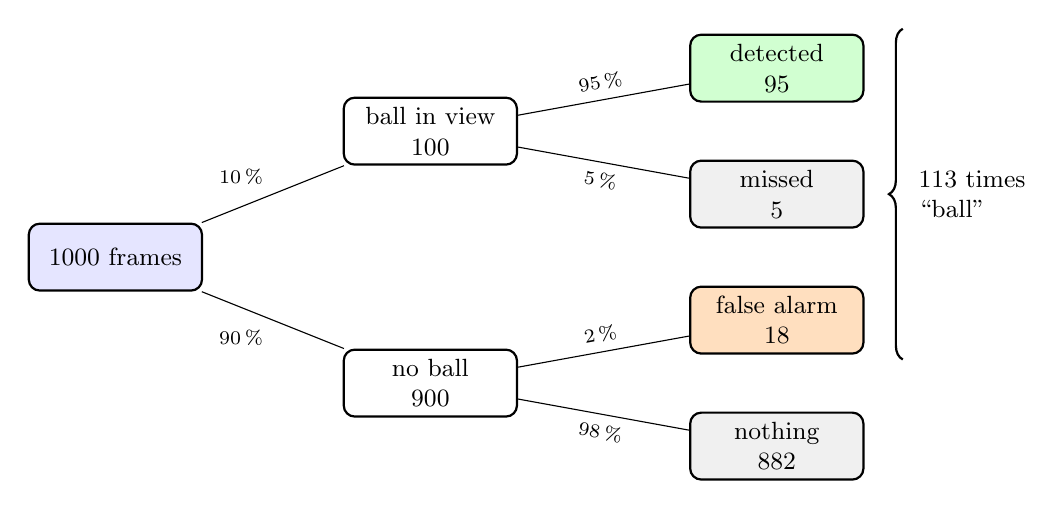
\begin{tikzpicture}[box/.style={draw,rounded corners,thick,align=center,font=\small,minimum height=0.85cm,minimum width=2.2cm},
  yes/.style={box,fill=green!18},no/.style={box,fill=gray!12},alarm/.style={box,fill=orange!25},
  every edge/.style={draw,-{Stealth},thick}]
  \node[box,fill=blue!10] (r) at (0,0) {$1000$ frames};
  \node[box] (b) at (4,1.6) {ball in view\\$100$};
  \node[box] (n) at (4,-1.6) {no ball\\$900$};
  \node[yes] (bd) at (8.4,2.4) {detected\\$95$};
  \node[no]  (bm) at (8.4,0.8) {missed\\$5$};
  \node[alarm] (nd) at (8.4,-0.8) {false alarm\\$18$};
  \node[no]  (nm) at (8.4,-2.4) {nothing\\$882$};
  \draw (r) -- node[above left,font=\scriptsize]{$10\,\%$} (b);
  \draw (r) -- node[below left,font=\scriptsize]{$90\,\%$} (n);
  \draw (b) -- node[above,font=\scriptsize,sloped]{$95\,\%$} (bd);
  \draw (b) -- node[below,font=\scriptsize,sloped]{$5\,\%$} (bm);
  \draw (n) -- node[above,font=\scriptsize,sloped]{$2\,\%$} (nd);
  \draw (n) -- node[below,font=\scriptsize,sloped]{$98\,\%$} (nm);
  \draw[thick,decorate,decoration={brace,amplitude=5pt,mirror}] (10.0,2.9) -- (10.0,-1.3) node[midway,right,xshift=2pt,font=\small,align=left]{$113$ times\\``ball''};
\end{tikzpicture}
\captionof{figure}{Counting with $1000$ frames. The detector says ``ball'' in $95+18=113$ frames, but only $95$ of them really contain the ball.}\label{fig:pr2_tree}
\end{center}

Among the $113$ frames with the answer ``ball'', only $95$ contain a ball:
\[
P(\text{ball}\mid\text{det})=\frac{95}{113}=0.841.
\]
So the robot should believe the detection with $84\,\%$, not with $95\,\%$. The reason: most frames contain no ball, so even a small false-alarm rate produces many false alarms ($18$ of $113$).

\begin{keyidea}[Do not mix up the direction]
$P(\text{det}\mid\text{ball})=0.95$ answers ``how often does the detector react if the ball is there?'' $P(\text{ball}\mid\text{det})=0.84$ answers ``how often is the ball there if the detector reacts?'' These are different questions with different answers.
\end{keyidea}

\subsection*{Bayes' rule}
What we just did by counting is \textbf{Bayes' rule}. Because $P(A\cap B)=P(B\mid A)P(A)$ and also $=P(A\mid B)P(B)$, we get
\[
P(A\mid B)=\frac{P(B\mid A)\,P(A)}{P(B)}.
\]
The denominator is computed with the \textbf{law of total probability}: if $A$ and $\bar A$ cover all cases,
\[
P(B)=P(B\mid A)P(A)+P(B\mid\bar A)P(\bar A).
\]
For the detector: $P(\text{det})=0.95\cdot0.10+0.02\cdot0.90=0.095+0.018=0.113$, so $P(\text{ball}\mid\text{det})=\frac{0.095}{0.113}=0.841$, the same as before.

The four parts have names that you will meet again in machine learning:
\begin{center}
\renewcommand{\arraystretch}{1.25}
\begin{tabular}{lll}
$P(A)$ & \textbf{prior} & what we believed before the measurement ($0.10$)\\
$P(B\mid A)$ & \textbf{likelihood} & how likely the measurement is if $A$ is true ($0.95$)\\
$P(B)$ & \textbf{evidence} & how likely the measurement is overall ($0.113$)\\
$P(A\mid B)$ & \textbf{posterior} & what we believe after the measurement ($0.841$)\\
\end{tabular}
\end{center}

\begin{example}[Fall alarm]
A falling robot is rare: $P(\text{fall})=0.01$ per time step. An alarm triggers with probability $0.99$ in a real fall, and with probability $0.05$ without a fall. The alarm just triggered. Then $P(\text{alarm})=0.99\cdot0.01+0.05\cdot0.99=0.0099+0.0495=0.0594$ and
\[
P(\text{fall}\mid\text{alarm})=\frac{0.0099}{0.0594}=\frac16\approx0.167.
\]
Only one alarm in six is a real fall, although the alarm detects $99\,\%$ of all falls! If falls are rare, even a good alarm gives mostly false alarms.
\end{example}

\subsection*{Updating a belief again and again}
The posterior of one measurement can become the prior of the next one. After the first detection the robot believes in the ball with $0.841$. A second detection in the next frame (assume the frames are independent given the situation) gives
\[
P(\text{ball})=\frac{0.841\cdot0.95}{0.841\cdot0.95+0.159\cdot0.02}=\frac{0.7987}{0.8019}=0.996.
\]
A third detection gives $0.9999$. Figure~\ref{fig:pr2_belief} shows how fast the belief grows. This repeated update is the core of the \textbf{Bayes filter}, the idea behind robot localisation: every new sensor reading sharpens the belief about the position. Single readings are unreliable, but many readings together are not.

\begin{center}
\begin{tikzpicture}
\begin{axis}[gr, width=9cm,height=5.2cm, xmin=-0.3,xmax=3.3, ymin=0,ymax=1.08, xtick={0,1,2,3}, ytick={0,0.25,0.5,0.75,1}, xlabel={number of detections in a row}, ylabel={belief $P(\text{ball})$}, axis lines=left, xlabel near ticks, ylabel near ticks, nodes near coords, every node near coord/.append style={font=\scriptsize,above right}]
  \addplot[thick,blue!60!black,mark=*] coordinates {(0,0.1) (1,0.841) (2,0.996) (3,0.9999)};
\end{axis}
\end{tikzpicture}
\captionof{figure}{Belief in the ball after repeated detections. The prior is $0.1$. A single detection brings it to $0.84$, three detections to $0.9999$.}\label{fig:pr2_belief}
\end{center}

\begin{aibox}
A neural network classifier outputs numbers that behave like probabilities: ``ball $0.84$, robot $0.10$, nothing $0.06$''. Bayes' rule explains why the prior matters. A network trained on images that are half balls and half non-balls will produce too many false alarms on a real match, where balls are rare. You will see in Chapter~\ref{ch:xent} how such outputs are trained. A \textbf{naive Bayes classifier} is a classic machine-learning method that applies Bayes' rule directly, and the particle and Kalman filters of Part~X are repeated Bayes updates.
\end{aibox}

\section*{Practice problems}
\begin{enumerate}[label=\textbf{\thechapter.\arabic*}]
  \item Two dice are rolled. Find (a) $P(\text{sum}=8\mid\text{first die}=2)$, (b) $P(\text{first die}=6\mid\text{sum}\ge11)$.
  \item In $200$ test frames, $80$ contained a ball and the detector found it in $72$ of them. Of the $120$ frames without ball, the detector gave a false alarm in $6$. Find $P(\text{det}\mid\text{ball})$, $P(\text{det}\mid\text{no ball})$ and $P(\text{ball}\mid\text{det})$.
  \item Are $A$ and $B$ independent? (a) $P(A)=0.5$, $P(B)=0.4$, $P(A\cap B)=0.2$. (b) $P(A)=0.5$, $P(B)=0.4$, $P(A\cap B)=0.3$.
  \item A bag contains $3$ red and $2$ blue balls. Two balls are drawn \emph{without} putting the first back. What is the probability that both are red?
  \item An alarm detects $98\,\%$ of the falls and gives a false alarm in $4\,\%$ of the time steps without fall. Falls occur with $P=0.02$. What is $P(\text{fall}\mid\text{alarm})$?
  \item Lighting is good in $70\,\%$ of the frames and bad in $30\,\%$. The ball is detected with probability $0.95$ in good light and $0.60$ in bad light (assume the ball is always in view). (a) What is the overall detection probability? (b) If the ball was detected, how likely was the light good?
  \item Using the detector of this chapter ($0.10$, $0.95$, $0.02$): after the first detection the belief is $0.841$. The next frame brings \emph{no} detection. Compute the new belief. (Use $P(\text{no det}\mid\text{ball})=0.05$ and $P(\text{no det}\mid\text{no ball})=0.98$.)
  \item In your own words: why is $P(\text{ball}\mid\text{det})$ smaller than $P(\text{det}\mid\text{ball})$ in the example of this chapter?
  \item Write a Python simulation with $1\,000\,000$ frames that estimates $P(\text{ball}\mid\text{det})$ for the detector of this chapter. What value do you expect?
  \item[\textbf{\thechapter.10}$\star$] (Monty Hall) A prize is behind one of three doors, chosen uniformly at random. You pick door~1. The host, who knows where the prize is, opens another door with a goat and offers to let you switch to the remaining door. Is switching better? Compute the winning probabilities by listing the three equally likely cases.
\end{enumerate}
